\section{Case Study}\label{ss:casestudy}

In this section, we present the results of applying our framework to static and dynamic personalization of apixaban dosing. \textbf{Insert apixaban data info/background.}

\subsection{Bayesian Modelling}

We extend a previously proposed one-compartment Bayesian pharmacokinetic model \cite{pananos2020comparisons} to include fixed effects of covariates on pharmacokinetic parameters in order to incorporate baseline clinical information (age, sex, weight, and creatinine.)  Full details of the model structure are provided in Appendix~\ref{ap:appendix}. We fit the model to previously-collected data on apixaban concentration \cite{tirona2018apixaban} and then use the fitted model to simulate patients with known "ground truth" pharmacokinetic parameters. We will then use this population of simulated patients in our experiments to explore different modes of dose personalization and their relative benefits.

\begin{figure}
	\centering
	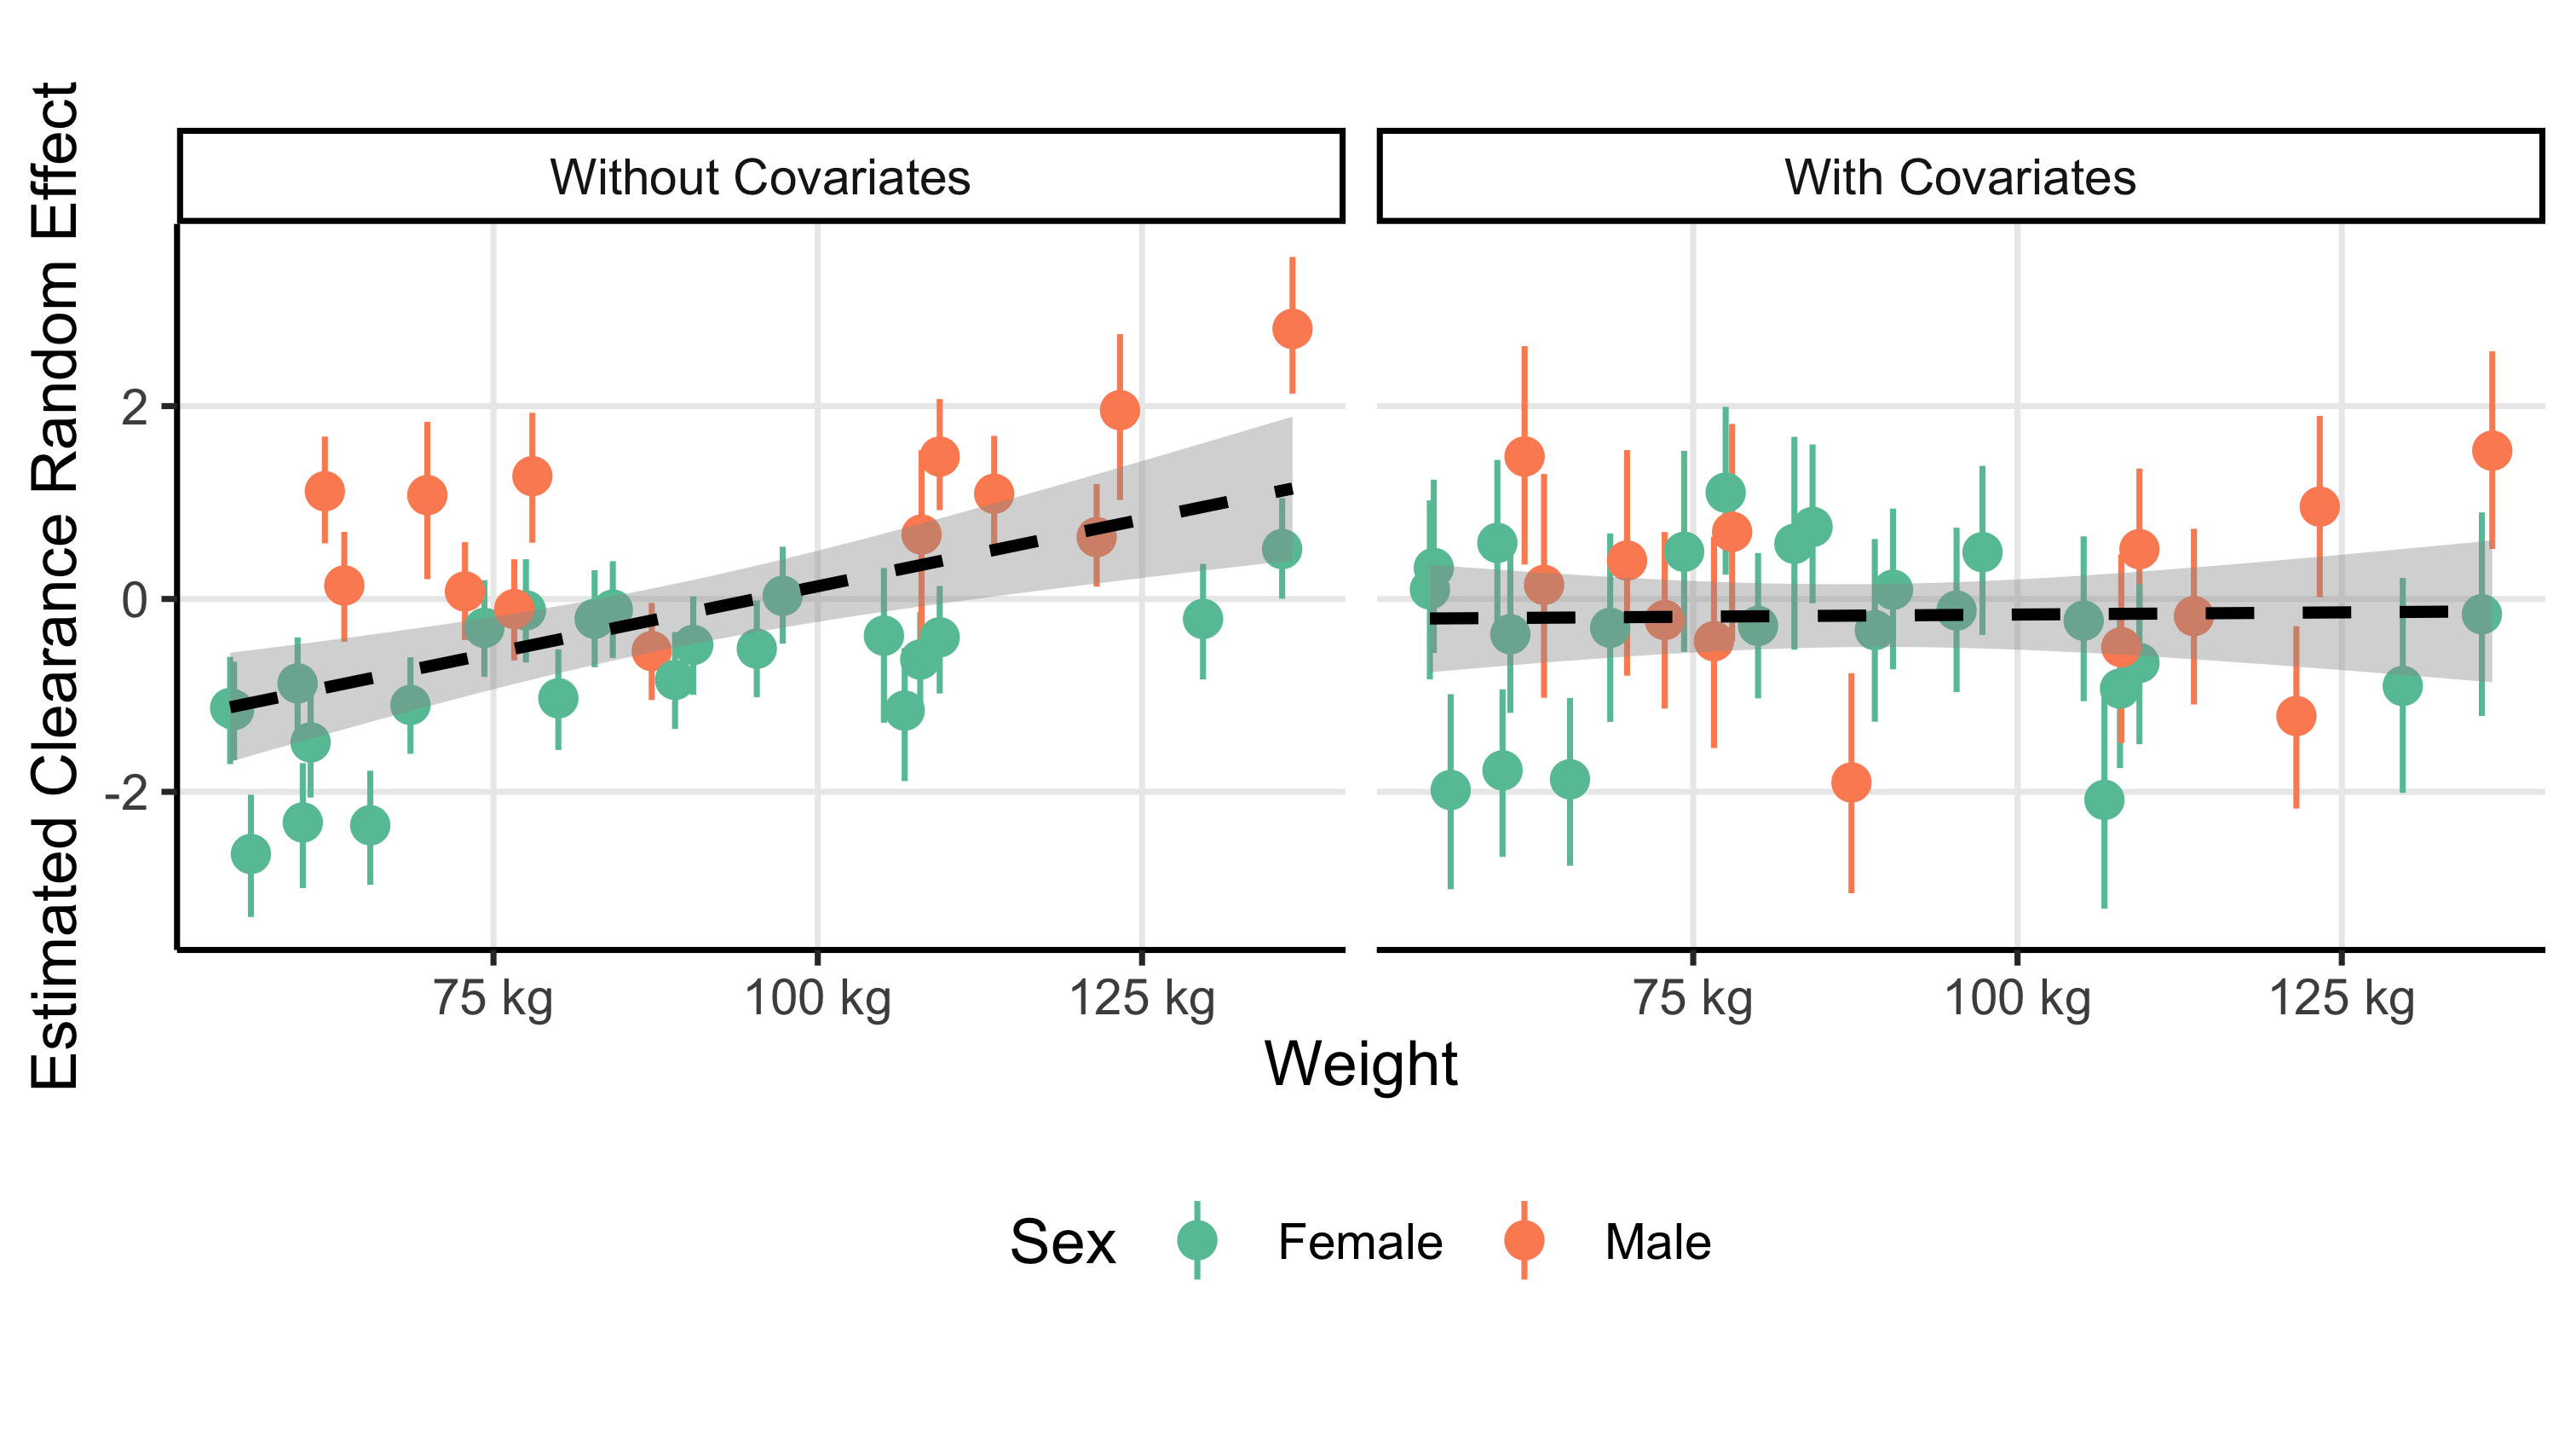
\includegraphics[width=\linewidth]{"figures/random_effects_change.png"}
	\caption{Random effects estimates for clearence rate $ Cl_i $ and 95\% credible intervals (left).  Random effects estimates are colored by patient sex.  Prior to adjusting for covariates, a general trend in weight can be seen in the random effects.  Subjects who are heavier tend to have larger random effect, and males tend to have larger random effects than females of the same weight.  Patterns such as these indicate that weight and sex can be used to explain variation in the random effects.  After adjusting for sex and weight (right), the random effects have no discernable pattern.}
	\label{fig:randomeffectschange}
\end{figure}
f
We fit M1 to real pharmacokinetic data using the Stan software in R\cite{}.  Stan monitors several markov chain diagnostics, none of which detected problematic markov chain behavior, which indicates that Stan’s sampling algorithm was able to converge to the target distribution (0 divergences, all all Gelman-Rubin diagnostics<1.01, all effective sample size ratios  > 22\%).  

The inclusion of covariates in the model results in a better fit than excluding them. Shown in \cref{fig:randomeffectschange} are the estimated random effects for the clearance pharmacokinetic parameter of each subject as a function of weight.  Subject sex is indicated by color, the overall trend is shown in the black dashed line.  Failing to include subject sex and weight results in males having on average a larger random effect than females of the same weight, and heavier subjects having a larger random effect than lighter subjects.  When covariates are added into the model, the variation in the random effects attenuates, resulting in closer alignment to model assumptions. A better fit to the data means data generate from the model may be closer aligned with the true data generating process.

Examining the posterior distributions of the regression coefficients provides further insights into the relationships between covariates and pharmacokinetics.  Subject weight increases the expected value of alpha (which is used to compute the elimination and absorption rates in the first order one compartment PK model.  The parameter $ \alpha $ is the ratio of how fast the drug exists the central compartment to how fast the drug enters the central compartment) as well as the time to max concentration.  There is an estimated effect of sex on $ \alpha $ (males have smaller alpha than females, meaning the drug leaves their central compartment slower or enters the central compartment quicker), however the uncertainty is large (estimated effect -0.2 on the logit scale, 95\% credible interval -0.54 to 0.15). \textcolor{red}{See Table~X} in the Appendix for a full summary of the regression coefficients.


\begin{figure}
	\centering
	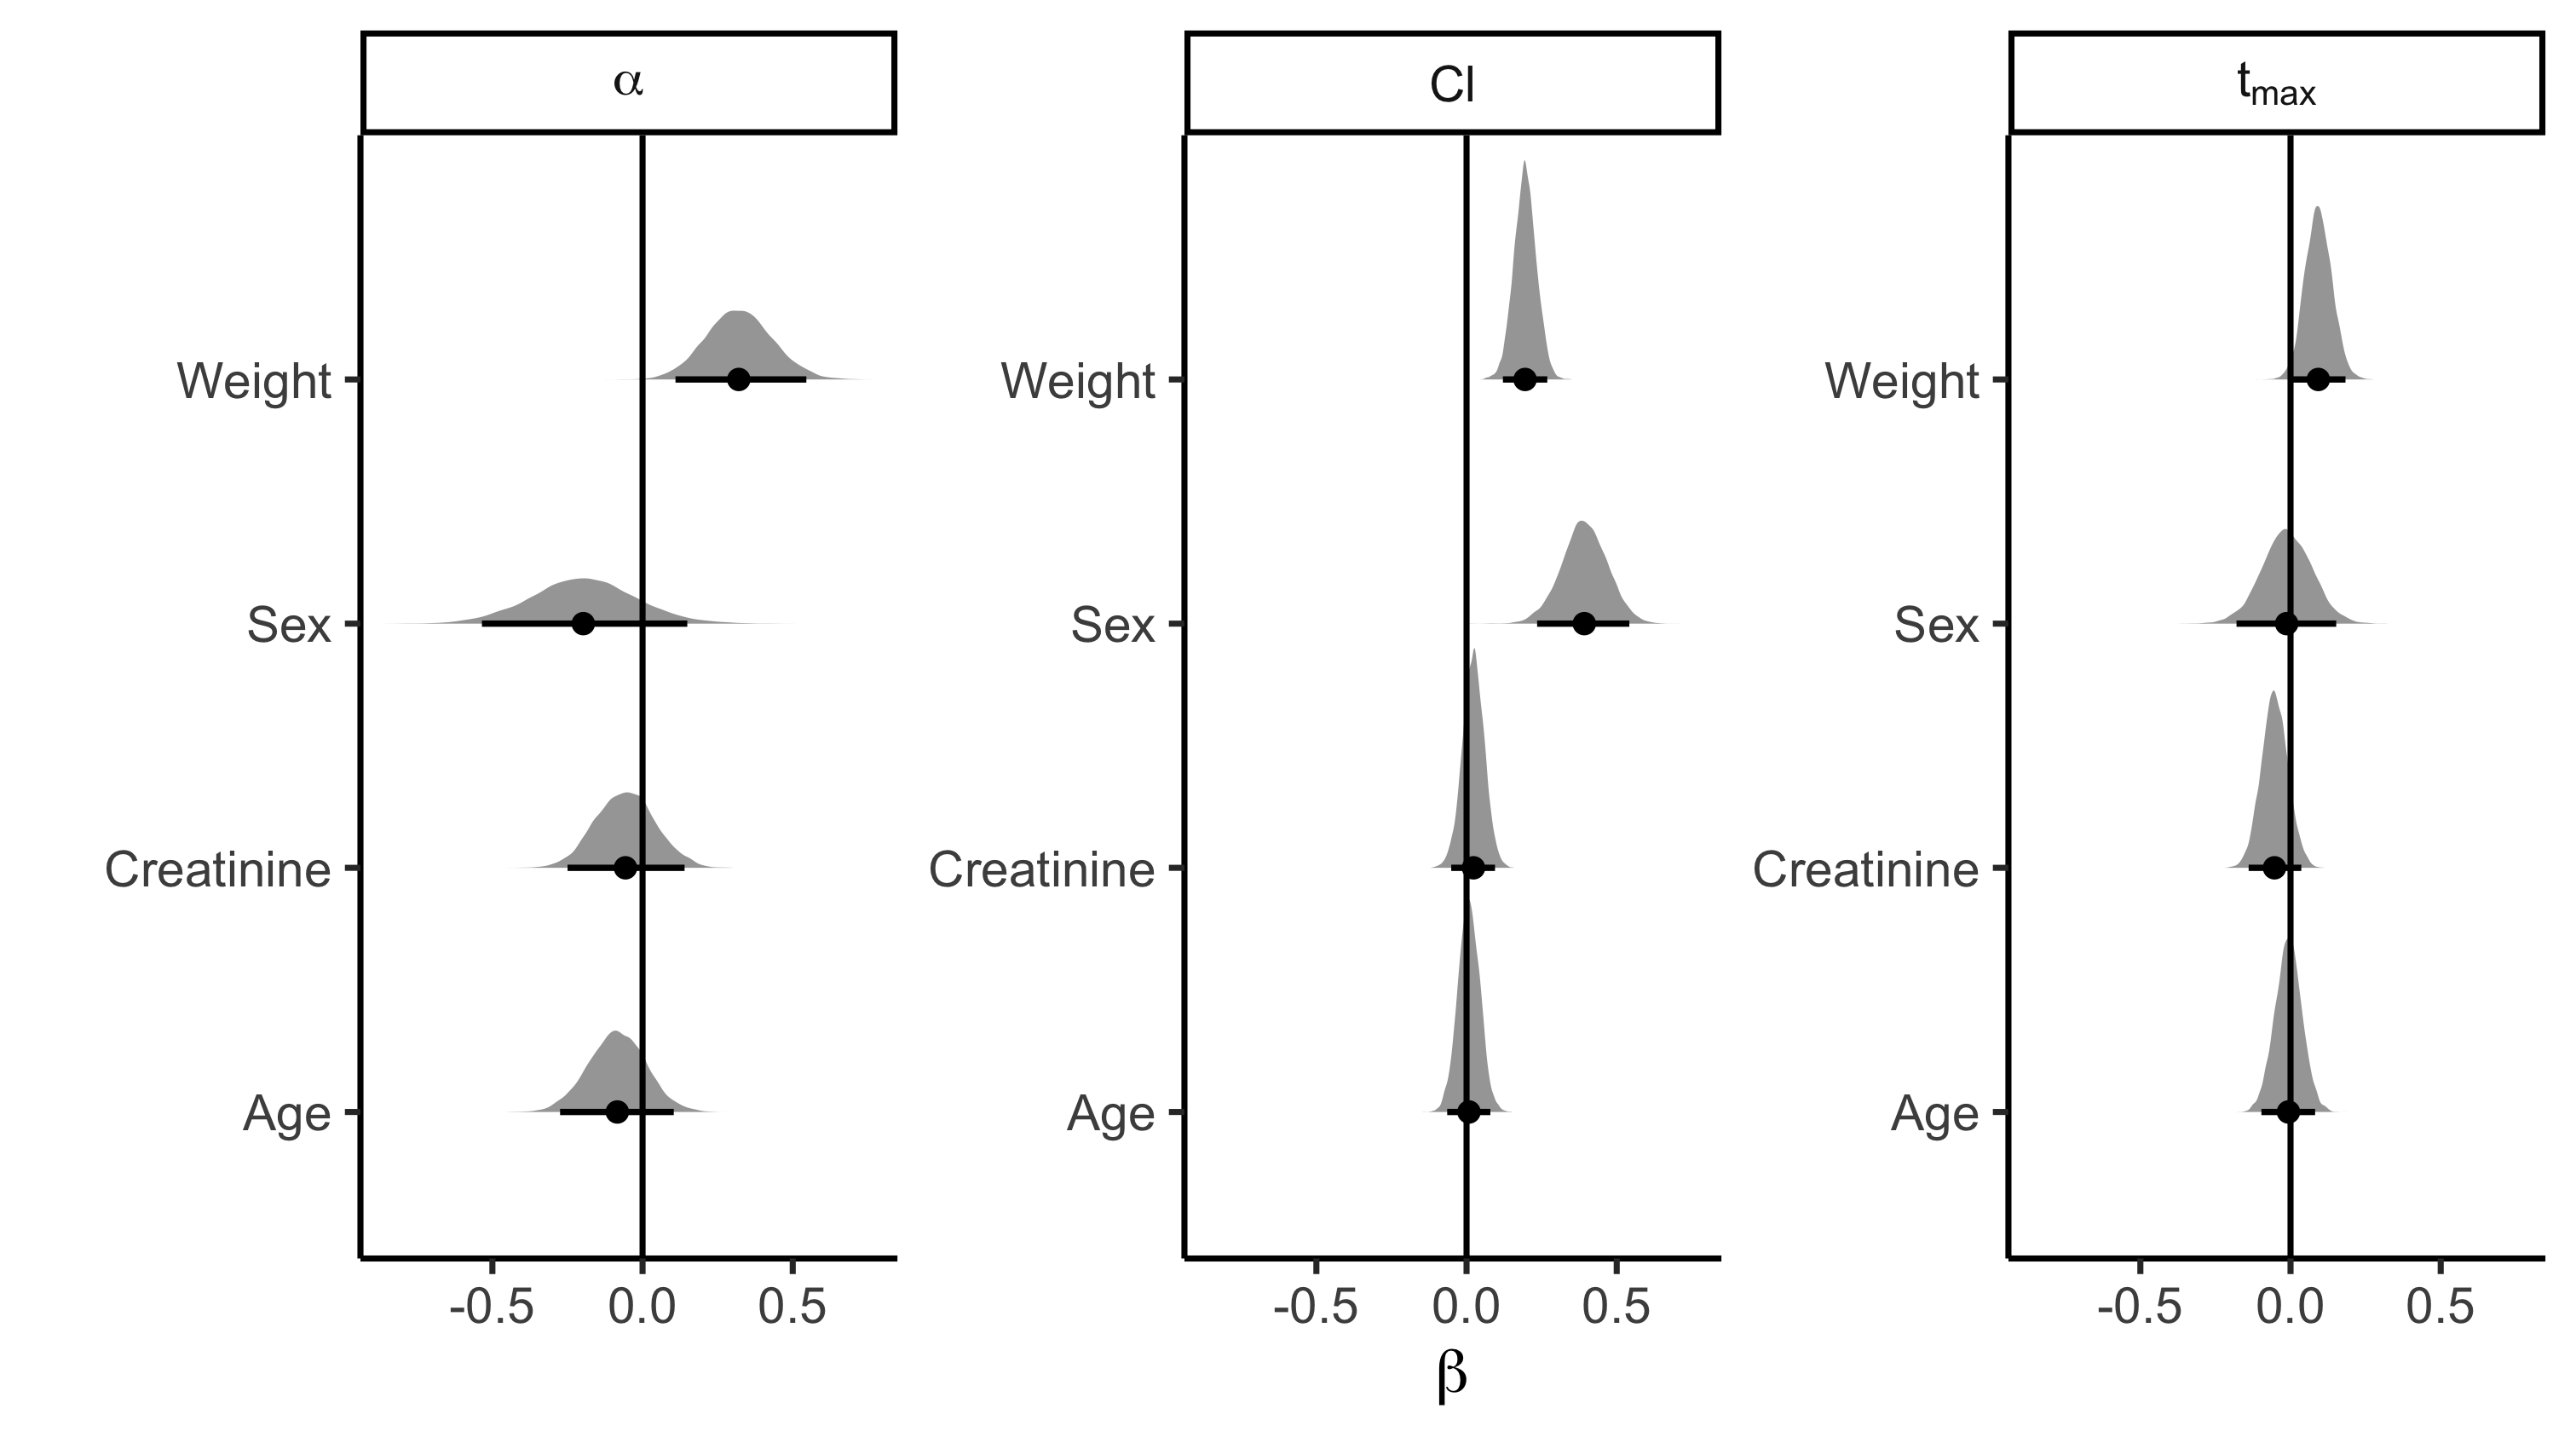
\includegraphics[width=1\linewidth]{figures/coef_vals}
	\caption{Posterior distributions of regression coefficients. Expectations are shown as black dots, 95\% credible intervals are shown as horizontal black lines.  Solid black vertical line is $\beta=0$ for reference.  Note, regression coefficients for $Cl$ and $t_{max}$ act multiplicatively (a one unit increase in weight leads to a change in $Cl$ of $\exp(\beta)$), while regression coefficients for $\alpha$ are interpreted on the log odds scale.}
	\label{fig:coefvals}
\end{figure}


Model training error sees a very small improvement.  Including subject covariates decreases model training error from 6.89 ng/ml to 6.84 ng/ml. Estimates of concentration uncertainty remain similar between the two models as well.  We conclude the inclusion of covariates in the model improves model inferences but does not improve the fit of the model to the data in any substantial way.  Either model would require additional validation prior to using in a predictive capacity.

\subsection{Modes of Personalization}

Implementing static and dynamic personalization as a dynamic treatment regime \citep{chakraborty2013statistical}, we propose six policies, each increasing in complexity and clinic/patient burden, for personalizing doses of apixaban with the goal of keeping blood serum concentrations within a desired range for as long as possible.

Thus far, we have motivated personalization of dose sizes through Q learning.  Q learning is the most complex solution that could be implemented at this time, and its implementation in practice would be burdensome due to this complexity. This makes implementation of Q learning a tall order, especially considering alternative DTRs exist which are not as costly to implement. The cost of implementing Q learning may be worth paying if the benefit of Q learning over these other DTRs is substantial, but we need a framework in which to estimate the size of this benefit. 

Our study considers the following modes of personalization. Each one has different requirements in terms of computation, data needs, clinical overhead, and patient burden. Our study aims to understand, in this particular setting (apixaban with potential PK monitoring) what the relative benefits of these different modes might be in practice. It also presents a general framework for evaluating these different modes of personalization in other settings.  The six modes of personalization we consider are:

\subsubsection{Experimental Design In Terms of Stages of a DTR}

In our experiments, we develop a DTR for selecting the best dose for keeping a patient’s blood plasma concentration within a desired range. Here, we present details of the experimental design in the DTR framework, leaving simulation details (including how the data were simulated) for our methods section.

Our experiment consists of 1000 simulated subjects taking a dose of apixaban once every 12 hours with perfect adherence for a total of 10 days.  Sometime in the second 12 hour period on the fourth day (between 108 and 120 hours after the initial dose), we have the opportunity to measure  the simulated subject’s blood concentration, should our policy allow for it.  At the start of the fifth day, the dose is adjusted based on all the pre-dose clinical measurements plus the observed concentration. The dose will be adjusted so as to attempt to maximize the time spent between 0.1 mg/L and 0.3 mg/L. Thus, our DTR consists of two stages (the first five days, and the latter five days), however the size of the range may be adapted for different scenarios. We choose this range as it is not so narrow that even optimal doses perform poorly, but not so wide that any dose can achieve high reward. 

In terms of the DTR, the system is the patient for whom a dose is selected, the actions correspond to selection of dose sizes, and the reward is the proportion of time spent within the desired concentration range. The trajectories we will use to estimate the optimal Q functions are of the form

\begin{equation}\label{key}
O_1, A_1, Y_1, O_2, A_2, Y_2, O_3
\end{equation}

\noindent The interpretation of a given trajectory is:
\begin{itemize}
	\item $ O_1 $ is any pre-dose clinical measurements of the subject.  In our experiments, we consider age in years, renal function (as measured by serum creatinine in mMol/L), weight in kilograms, and dichotmous biological sex (dummy coded so that male=1 and female=0).  We choose these variables as they are known to affect the pharmacokinetics of apixaban \cite{byon2019apixaban}.  
	\item $ A_1 $ is dual action of initial dose to provide the subject plus a time in the future at which to measure the subject’s blood serum concentration.
	\item $ Y_1 $ is the proportion of time spent within the concentration range in the first five days.
	\item $ O_2 $ is the pre clinical measurements of the subject plus the observed concentration made on the fourth day.
	\item $ A_2 $ is the dose adjustment
	\item $ Y_2 $ is the proportion of time spent within the concentration range in the last five days after the dose adjustment.
	\item $ O_3 $ would be pre-dose clinical measurements, the observed concentration made on the fourth day, and the next concentration measurement, were it to be made. As we examine just the two actions $ A_1 $ and $ A_2 $, we do not make use of $ O_3 $ but include it here to adhere with our definition of trajectories above.
\end{itemize}

The reward function we use depends on the subject’s true latent concentration. Let $ c_j \quad j=1...K $ be the $ j^{th}$ latent concentration value at time $ t_j $.  The reward function is 

\begin{equation}
Y(c_1, c_2, \cdots, c_k) = \dfrac{1}{k}\sum_{j=1}^K \mathbb{I}(0.1 < c_j < 0.3)
\end{equation}

\noindent Here, $ \mathbb{I} $ is an indicator function returning 1 if the argument is true, and 0 else.  
%To leverage off-the-shelf optimization tools, we approximate this reward function with a continuously differentiable function, namely
%\begin{equation}
%Y(c_1, c_2, \cdots,  c_k) = \dfrac{1}{k}\sum_{j=1}^K \exp\left( - \left[ \dfrac{c_j-0.15}{0.05} \right]^{2\beta} \right)
%\end{equation}
%
%\noindent Here, $ \beta $is a positive integer.  For sufficiently large beta, our approximation becomes arbitrarily close to our intended reward function.  In practice we set beta=5 to balance between good approximation of our intended reward and vanishing gradients impeding our optimization. 
We suppress the dependence on the history in the definition of the reward as the reliance on the history is implicit.  The reward depends on the latent concentrations which depend on previous doses (actions) and potentially on the previous dose measurements (observations of the system).  We approximate this reward function with a continuously differentialble function to facilitate optimization.  See the appendix for details.  

Our stage 2 optimal Q function is then

\begin{equation}
Q_{2}^{o p t}\left(H_{2}, A_{2}\right)=E\left[Y\left(c_{j+1}, c_{j+2}, \cdots, c_{j+n}\right) \Bigg\vert H_{2}, A_{2}\right] \>,
\end{equation}

\noindent and our stage 1 optimal Q function is

\begin{equation}
Q_{1}^{o p t}\left(H_{1}, A_{1}\right)= E \left[Y\left(c_{1}, c_{2}, \cdots, c_{j}\right)+\max _{a_{2} \in \mathscr{A}} Q_{2}^{o p t}\left(H_{2}, a_{2}\right) \Bigg\vert H_{1}, A_{1}\right]
\end{equation}

We seek to maximize the stage 1 optimal Q function to learn the optimal policy for dosing subjects under the constraint we can measure them at most once and are limited to the aforementioned pre-dose clinical variables.  The interpretation of stage 1 optimal Q function is as follows:\textit{ Given the pre-dose clinical variables of the subject and a proposed initial dose and measurement time, the stage 1 optimal Q function gives the proportion of time the subject’s blood serum concentration is between 0.1mg/L and 0.3mg/L assuming that we provide the subject with the best dose possible at the start of the $ 5^{th} $ day.}  The actions $ A_1 $ and $ A_2 $ which maximize these functions constitute the optimal policy.

The concentration values $ c_j $ in the optimal Q functions are latent, meaning we have no direct access to them in practice. Furthermore, obtaining measurements with high enough frequency so that the reward is faithfully estimated would be too burdensome on the patient. 


We consider 6 modes of personalization which range in the amount of information used in the decision process as well as burden placed on the patient and clinic, and burden of implementation.  We present the results of our simulation in figure X below in terms of difference between theoretically largest reward and reward achieved by the mode of personalization.  The results are ordered from least amount of information and burden (top) to most amount of information and burden (bottom).

\begin{enumerate}[1)]
\item Dose selection using a hierarchical Bayesian model which does not incorporate subject covariates.  This model was presented in Pananos \& Lizotte \cite{pananos2020comparisons}.  We refer to this mode as the “No Covariate Model”.
\item 1) and conditioning the model on a single sample from the subject taken sometime in the final 12 hours before the half way point.  At the start of the fifth day, a new dose is selected and used for the remaining time.  We refer to this mode as “No Covariate + 1 Sample”.
\item Dose selection from M2.  A single dose is selected at the start of the regiment and is used throughout the 10 simulated days. We refer to this mode as “Covariate Model”.
\item 3) and conditioning the model on a single sample from the subject taken sometime in the final 12 hours before the half way point.  At the start of the fifth day, a new dose is selected and used for the remaining time. We refer to this mode as “Covariate model + 1 Sample”.
\item A two stage DTR, however the initial dose is the result of the procedure in 3).  The best time to sample the patient is then determined via Q learning. We refer to this mode as “Optimal Sampling Time”.
\item The two stage DTR we describe in the previous sections, estimated via Q learning.  We refer to this mode as “Q Learning”.
\end{enumerate}


\subsection{Evaluation of Benefits}

Modes of personalization which use less information have a larger difference (i.e. yield smaller reward on average than what is theoretically possible).  The no covariate model (which uses no information about the subject) performs worst with a median difference of 0.19.  The distribution of differences for this mode is right skewed with some differences exceeding 0.95, meaning the subject could have been in range for nearly the entire time but the mode selected a dose which failed to put the subject in range. 

The use of covariates in the model nearly cuts the difference in half, achieving an average difference of 0.1 with smaller right skew.  There is a diminishing in the difference in rewards as additional burden is undertaken. Modes which use observed concentration information (Covariate Model + 1 Sample, Optimal Sampling Time, and Q Learning) lead to marginally more reward on average.


\begin{figure}
	\centering
	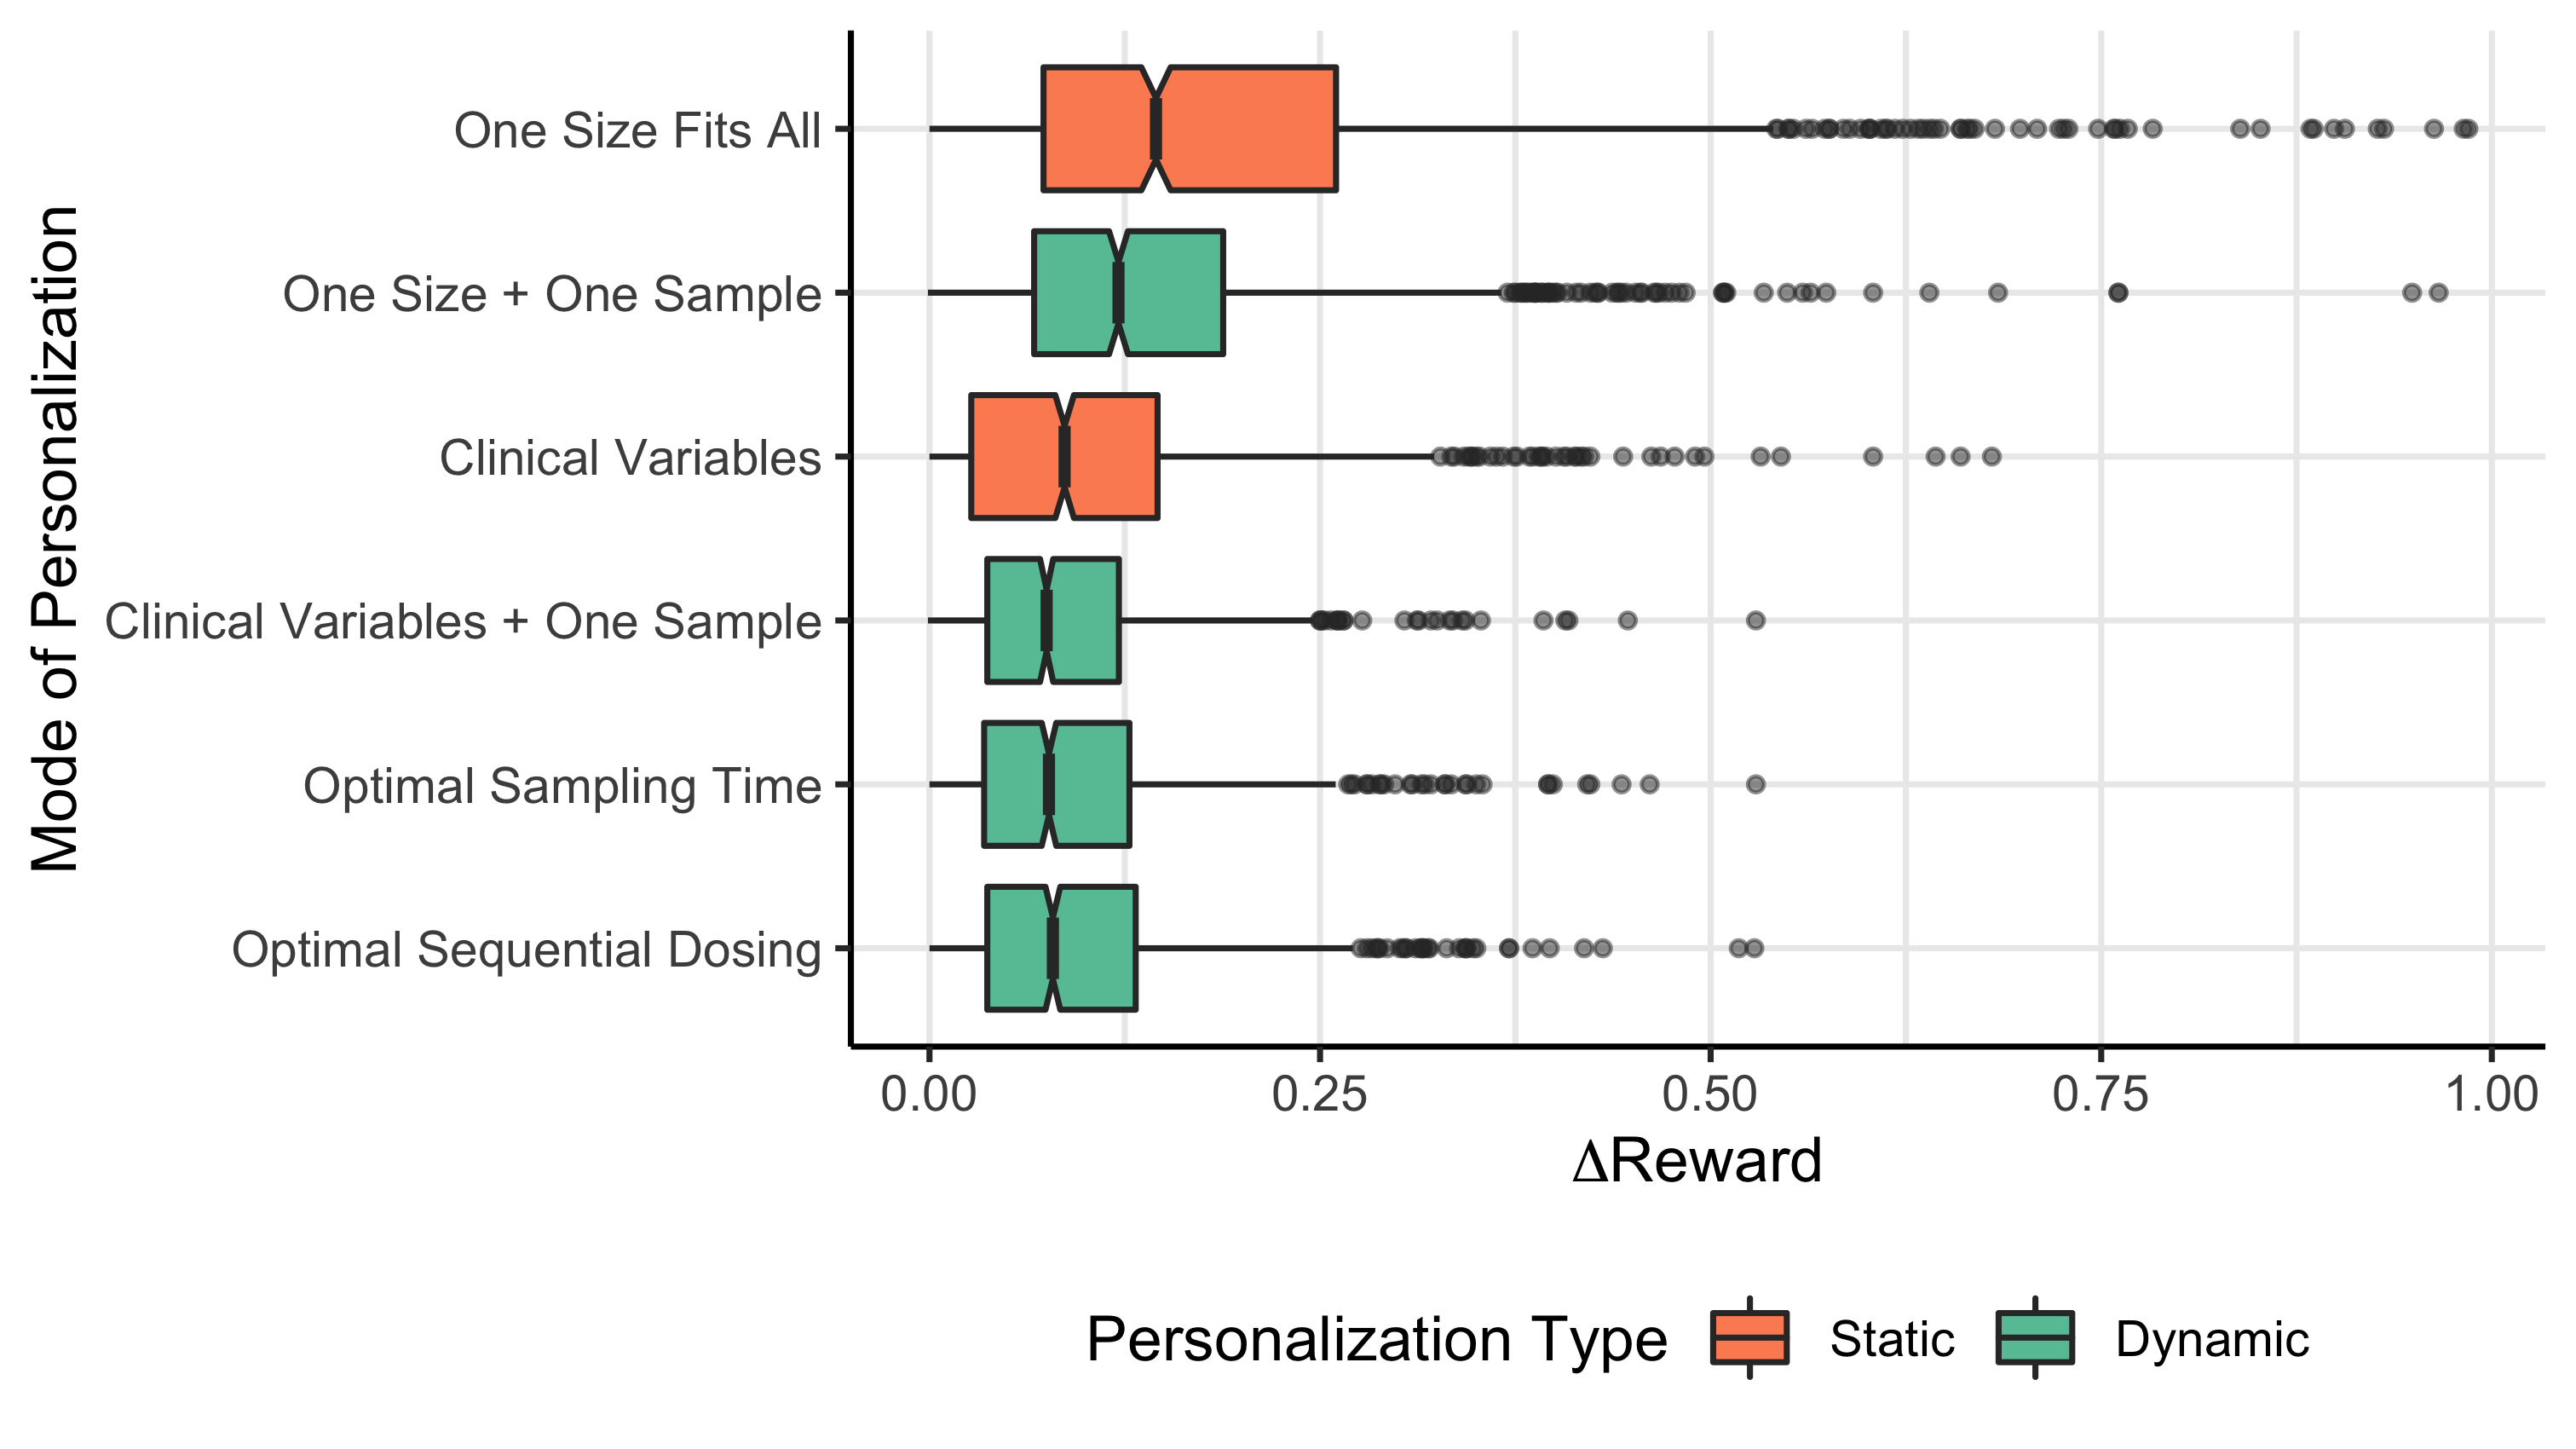
\includegraphics[width=1\linewidth]{figures/models_of_personalization_differences}
	\caption{Boxplots of the difference between theoretically largest reward and achieved reward for each of the 1000 simulated subjects. Subjects who achieve a reward close to their maximium reward have a difference on 0, subjects who achieve a reward less than their maximum have larger differences, with the largest difference being 1.}
	\label{fig:modelsofpersonalizationdifferences}
\end{figure}
